% EAJ - svg generation needs to be run with -shell-escape:
% pdflatex -shell-escape filename.tex
\documentclass[border=5pt,tikz, convert={pdf2svg,outfile=\jobname.svg}]{standalone}
\begin{document}
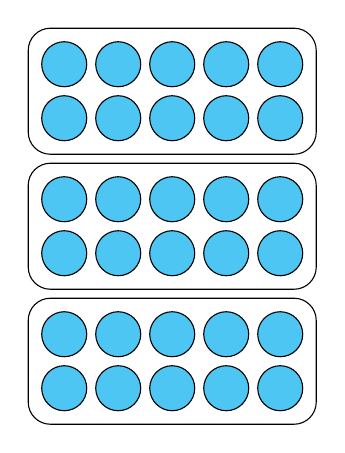
\begin{tikzpicture}[x=0.9in,y=0.9in]
% \foreach \shift in {(0,0),(0,-.65),(0,-1.3)}{
    \begin{scope}[shift={(0,0)}]
    \foreach \x in {0,.3,.6,-.3,-.6}{
        \foreach \y in {.15,-.15}{
            \draw[fill=cyan!70] (\x,\y) circle (.125);
        }}
    \draw[rounded corners=8pt] (-.8,-.35)rectangle(.8,.35);
    \end{scope}

    \begin{scope}[shift={(0,-.75)}]
    \foreach \x in {0,.3,.6,-.3,-.6}{
        \foreach \y in {.15,-.15}{
            \draw[fill=cyan!70] (\x,\y) circle (.125);
        }}
    \draw[rounded corners=8pt] (-.8,-.35)rectangle(.8,.35);
    \end{scope}

    \begin{scope}[shift={(0,-1.5)}]
    \foreach \x in {0,.3,.6,-.3,-.6}{
        \foreach \y in {.15,-.15}{
            \draw[fill=cyan!70] (\x,\y) circle (.125);
        }}
    \draw[rounded corners=8pt] (-.8,-.35)rectangle(.8,.35);
    \end{scope}
% }
\end{tikzpicture}
\end{document}